\documentclass[11pt]{standalone}
\usepackage{amssymb}
\usepackage{amsmath}
\usepackage[no-math]{fontspec}
\usepackage{unicode-math}
\usepackage{libertinus}
\usepackage{pgf,xcolor}
\usepackage{tikz}
\usetikzlibrary{arrows.meta, backgrounds}
\usepackage{pgfplots}
\pgfplotsset{compat=newest}

\definecolor{my_darkgray}{HTML}{484949}
\definecolor{my_lightgray}{HTML}{F3F4F4}
\definecolor{my_darkblue}{HTML}{005A94}
\definecolor{my_lightblue}{HTML}{CCDEE9}
\definecolor{my_yellow}{HTML}{FFEC7F}
\definecolor{my_red}{HTML}{E60000}
\definecolor{my_orange}{HTML}{E87846}

\begin{document}
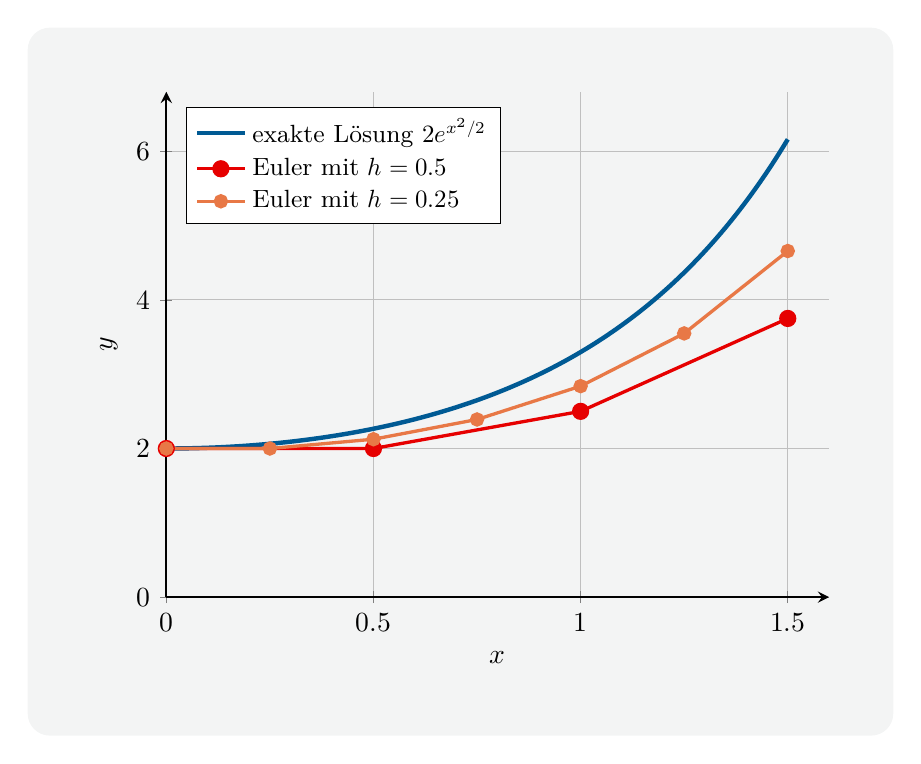
\begin{tikzpicture}[
    show background rectangle,
    background rectangle/.style={fill=my_lightgray, rounded corners=8pt},
    inner frame sep=0.8cm
]
% ---------------------------------------------------------------
%  AWP y' = x y, y(0) = 2, exakte Loesung y = 2 e^{x^2/2}
%  Euler h = 0.5:  2, 2, 2.5, 3.75
%  Euler h = 0.25: 2, 2, 2.125, 2.3906, 2.8389, 3.5486, 4.6575
%  axis equal weggelassen: y-Werte bis 6.2 bei x-Werten bis 1.5 waeren
%  bei gleicher Skalierung viermal so hoch wie breit.
% ---------------------------------------------------------------
\begin{axis}[
    axis lines = left,
    xlabel = {$x$},
    ylabel = {$y$},
    grid = both,
    axis line style={thick},
    width=10cm, height=8cm,
    xmin=0, xmax=1.6,
    ymin=0, ymax=6.8,
    xtick={0, 0.5, 1, 1.5},
    xticklabels={$0$, $0.5$, $1$, $1.5$},
    ytick={0, 2, 4, 6},
    legend pos=north west,
    legend style={font=\small},
    legend cell align=left,
]
\addplot[draw=my_darkblue, samples=300, ultra thick, domain=0:1.5]
    {2*exp(x^2/2)};
\addlegendentry{exakte Lösung $2e^{x^2/2}$}
\addplot[draw=my_red, very thick, mark=*, mark size=2.5pt,
    mark options={fill=my_red}]
    coordinates {(0, 2) (0.5, 2) (1, 2.5) (1.5, 3.75)};
\addlegendentry{Euler mit $h = 0.5$}
\addplot[draw=my_orange, very thick, mark=*, mark size=2pt,
    mark options={fill=my_orange}]
    coordinates {(0, 2) (0.25, 2) (0.5, 2.125) (0.75, 2.3906) (1, 2.8389)
                 (1.25, 3.5486) (1.5, 4.6575)};
\addlegendentry{Euler mit $h = 0.25$}
\end{axis}
\end{tikzpicture}
\end{document}
